%------------------------------------------%
% Cannabis Data Science #73
% Copyright (c) 2022 Cannlytics
% Date: 7/6/2022
%------------------------------------------%
\documentclass[xcolor={dvipsnames}]{beamer}
\hypersetup{pdfpagemode = FullScreen}
\mode<presentation>{
  \usetheme{Boadilla}
  \usecolortheme{orchid}
  \usefonttheme{default}
  \setbeamertemplate{navigation symbols}{}
  \setbeamertemplate{caption}[numbered]
}
\setbeamersize{
  text margin left = 0.5in,
  text margin right = 0.5in
}

%------------------------------------------%
% Title
%------------------------------------------%
\title[\textbf{Cannabis Data Science \#73}]{}
\author{Cannlytics}
\institute[]{\Large Cannabis Data Science \#73}
\date{July \nth{6}, 2022}

%------------------------------------------%
% Packages
%------------------------------------------%
\usepackage[english]{babel}
\usepackage[utf8x]{inputenc}
\usepackage{tikz} % For styling.
\usepackage{xparse}
\usepackage{amsmath}
\renewcommand*\footnoterule{} % No footnote line.
\usepackage{mathtools} % Annotating equations.
\usepackage{hhline} % Double bars.
\usepackage[super]{nth} % 1st, 2nd, 3rd, etc.
\usepackage{graphicx, caption, subcaption}
\usepackage{setspace}
\usepackage[charter]{mathdesign}
\usepackage{tikz}
\usetikzlibrary{tikzmark}
\usetikzlibrary{arrows.meta}

%------------------------------------------%
% Theme
%------------------------------------------%
\definecolor{LG}{RGB}{218, 247, 166}
\definecolor{DG}{RGB}{2, 48, 32}
\setbeamercolor*{palette primary}{bg=LG, fg=DG}
\setbeamercolor*{palette secondary}{bg=LG, fg=DG}
\setbeamercolor*{palette tertiary}{bg=LG, fg=DG}

%------------------------------------------%
% Commands
%------------------------------------------%

% Top space.
\newcommand\T{\rule{0pt}{2.5ex}}

% Bottom space.
\newcommand\B{\rule[-1.25ex]{0pt}{0pt}}

% Blocks.
\newenvironment<>{Block}[2][.9\textwidth]
  {\setlength{\textwidth}{#1}
  \begin{actionenv}#3
    \def\insertblocktitle{#2}\par
    \usebeamertemplate{block begin}}
  {\par\usebeamertemplate{block end}
  \end{actionenv}}

% Balls.
\defbeamertemplate{enumerate item}{largeball}
{\begin{pgfpicture}{-1ex}{-0.65ex}{1.5ex}{1.5ex}
\usebeamercolor[fg]{item projected}
{\pgftransformscale{2.5}\pgftext{\Large\pgfuseshading{bigsphere}}}
{\pgftransformshift{\pgfpoint{0pt}{0.5pt}}
\pgftext{\usebeamerfont*{item projected}\small\insertenumlabel}}
\end{pgfpicture}}

% Fancy arrows.
\NewDocumentCommand\UpArrow{O{2.0ex} O{black}}{%
   \mathrel{\tikz[baseline] \draw [->, line width=0.5pt, #2] (0,0) -- ++(0,#1);}} % Fancy up-arrow.
\NewDocumentCommand\DownArrow{O{2.0ex} O{black}}{%
   \mathrel{\tikz[baseline] \draw [<-, line width=0.5pt, #2] (0,0) -- ++(0,#1);}} % Fancy down-arrow.

% Equations with numbers on the left.
\makeatletter
\newcommand{\LeftEqNo}{\let\veqno\@@leqno}
\makeatother

% Print out title.
\defbeamertemplate*{title page}{customized}[1][]
{
  \usebeamerfont{title}\inserttitle\par
  \bigskip
  \vspace{0.5\baselineskip}
  \usebeamerfont{institute}\insertinstitute\par
  \vspace{0.5\baselineskip}
  {\small\usebeamerfont{date}\insertdate\par}
  \usebeamercolor[fg]{titlegraphic}\inserttitlegraphic
}

%------------------------------------------%
%
% Presentation
%
%------------------------------------------%
\begin{document}

% Title page.
\begin{frame}{}

% Background
\tikz[remember picture, overlay]
\node[opacity=1.0, inner sep=0pt] at (current page.center){
  
\includegraphics[height=\paperheight, width=\paperwidth]{images/presentation-cover.pdf}
};

% Title
\vspace*{4\baselineskip}

\includegraphics[scale=0.375]{images/logo.pdf}
\vspace*{-2\baselineskip}
\titlepage
\end{frame}

%------------------------------------------%
% Icebreaker
%------------------------------------------%

\begin{frame}{}

\begin{center}
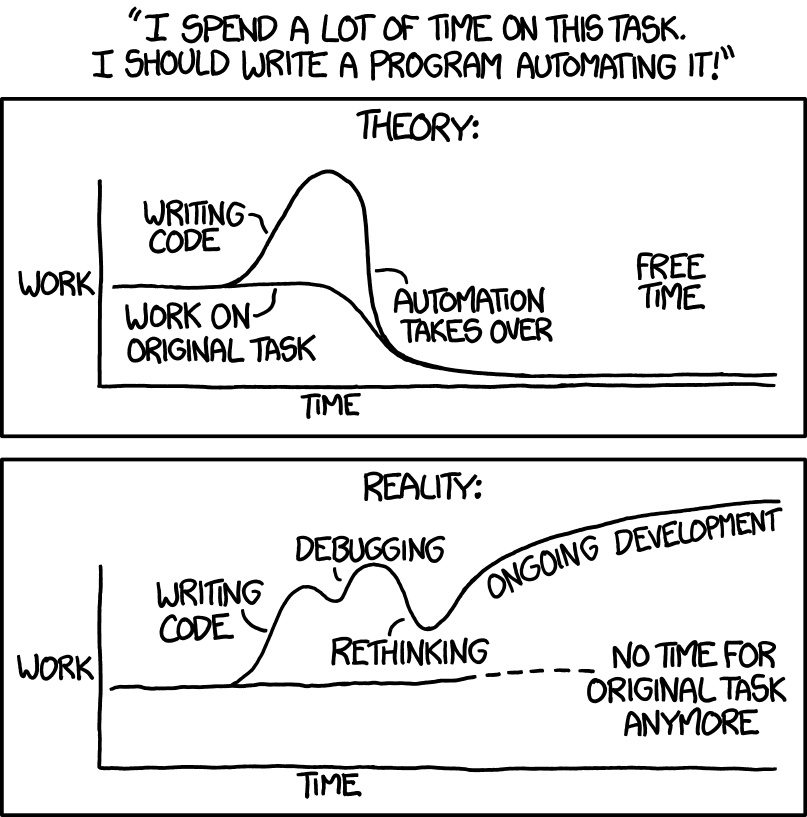
\includegraphics[width=3in]{images/automation-xkcd.png}\\
\begin{flushleft}
{\tiny Author: xkcd\\
License: CC BY-NC 2.5\\[-0.75\baselineskip]
URL: https://xkcd.com/1319/}
\end{flushleft}
\end{center}

\end{frame}

%------------------------------------------%
% Introduction
%------------------------------------------%


\begin{frame}{Topics of the day}

\begin{minipage}{0.45\textwidth}

\vspace{0.5\baselineskip}
\begin{itemize}

\item {\bfseries Web scraping}

\vspace{0.5\baselineskip}

\item {\bfseries Margin of error}

\vspace{0.5\baselineskip}

\item {\bfseries Secure Hash Algorithms or SHA256}

\vspace{0.25\baselineskip}
\begin{itemize}

\item Developed by the NSA (2002).

\vspace{0.25\baselineskip}

\item The underlying technology of {\bfseries Bitcoin}!

\end{itemize}

\end{itemize}

\end{minipage}\hspace{0.025\textwidth}%
\begin{minipage}{0.45\textwidth}

\begin{center}
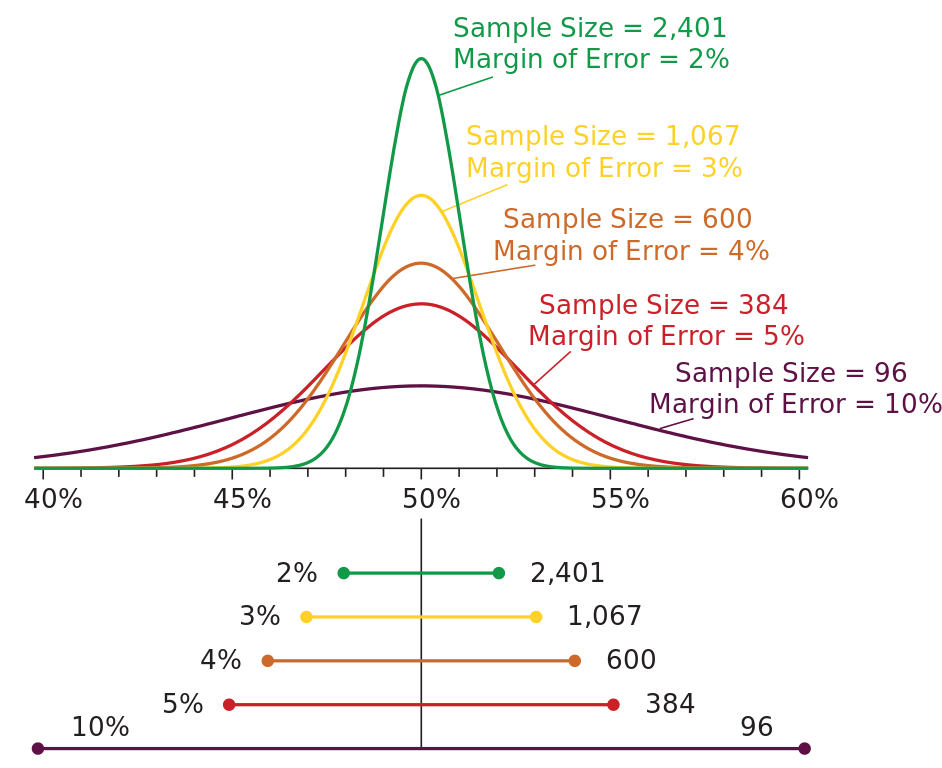
\includegraphics[width=2in]{images/margin-of-error.png}\\
\begin{flushleft}
{\tiny Author: Zieben007\\
License: CC BY-NC 3.0\\[-0.75\baselineskip]
https://creativecommons.org/licenses/by-sa/3.0}
\end{flushleft}
\end{center}

\end{minipage}

\end{frame}


%------------------------------------------%
% Scientific Process
%------------------------------------------%

%\begin{frame}{Scientific Process}
%
%\begin{enumerate}
%
%\item {\bfseries Hypothesis}
%
%\vspace{0.5\baselineskip}
%
%\item Literature Review
%
%\vspace{0.5\baselineskip}
%
%\item Methodology
%
%\vspace{0.5\baselineskip}
%
%\item Data
%
%\vspace{0.5\baselineskip}
%
%\item Results
%
%\vspace{0.5\baselineskip}
%
%\item Conclusion
%
%\end{enumerate}
%
%\end{frame}



%------------------------------------------%
% Takeaway
%------------------------------------------%
\section{Takeaway}

\begin{frame}{}

\begin{center}
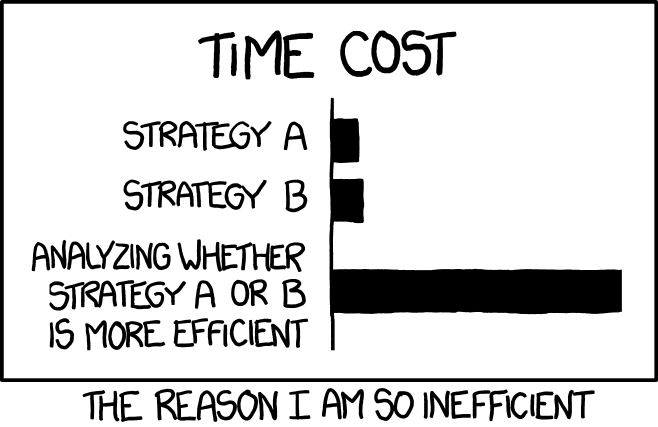
\includegraphics[width=3in]{images/efficiency-xkcd.png}\\
\begin{flushleft}
{\tiny Author: xkcd\\
License: CC BY-NC 2.5\\[-0.75\baselineskip]
URL: https://xkcd.com/1319/}
\end{flushleft}
\end{center}

\end{frame}

\begin{frame}{}

\vspace{0.5\baselineskip}

\begin{center}
\begin{minipage}{3.85in}

% Thank you.

\includegraphics[width=.25in]{images/prayer.png} {\Large \textbf{Thank you for coming.}}\\[-0.75\baselineskip]

\begin{center}
\begin{minipage}{\linewidth}
\begin{Block}{Insights of the Day}

\vspace{0.5\baselineskip}

\begin{itemize}

\item Automate the boring stuff!

\vspace{0.5\baselineskip}

\item Archive \underline{\bfseries all} the data.

\vspace{0.75\baselineskip}

\end{itemize}

\end{Block}
\end{minipage}
\end{center}

\vfill

\end{minipage}
\end{center}

\vspace{0.5\baselineskip}

{\large What is on your mind for next week?}\\

\end{frame}


%------------------------------------------%
% Fin.
%------------------------------------------%
\end{document}
